\chapter[Kernel-based Regularization for\\ Inducing Structured Sparsity in Transport Plans]{Kernel-based Regularization for Inducing \\Structured Sparsity in Transport Plans}
\label{chap:ch2}
\section{Introduction}\label{sec:sot-intro}
In this chapter, we demonstrate how the proposed kernel-based regularization to learn finitely parameterized OT plans (presented in Chapter~\ref{chap:ch1}) facilitates solutions with controlled structured sparsity.
We begin by showing that when one uses squared-MMD regularization to (softly) match the marginals in the OT formulation, the resulting objective becomes strongly convex and smooth. Leveraging this key property, we recast the problem of learning an OT plan with sparsity constraints to that of a submodular maximization problem.

As discussed in the previous chapters, the \textit{optimal value} of the optimization problem in OT, under mild conditions, yields a metric over measures. In Chapter~\ref{chap:ch1}, we focused on studying such metric-related properties. The \textit{optimal solution} of the OT optimization problem, called the optimal transport plan, also finds various applications in ML as a tool for distribution-aware alignment between sets, like aligning words in two sentences \citep{arase-etal-2023-unbalanced}, for semantic correspondence between objects in an image \citep{liu2020semantic} or for aligning points in the source and target data for domain adaptation \citep{Courty17domAda}.

In Sec.~\ref{bg:comp}, we discussed how the entropy-regularized OT formulation
\citep{cuturi13a} facilitates solving large-scale OT problems that typically arise in ML applications. The resulting OT problem not only becomes a differentiable convex program but also has an unconstrained dual optimization that can be solved with the Sinkhorn algorithm involving fast and parallelizable matrix-vector multiplications. 
However, a notable drawback of entropic regularization is that it renders a dense transport plan with strictly positive entries \citep{blondel18a,liu2023sparsityconstrained}. While lowering the entropic regularization coefficient ($\epsilon$) would alleviate this issue, a lower $\epsilon$ also slows down the convergence rate (Fig.~\ref{fig:entr-sparsity}) besides leading to numerical issues due to $(1/\epsilon)$ factors in the Sinkhorn algorithm (Sec. \ref{entOT}, \citep[Remark (4.7)]{peyre2019computational}).
\begin{figure}[ht]
    \centering
    \begin{tabular}{ccc}
        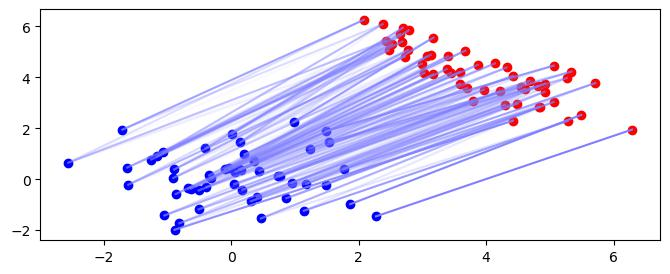
\includegraphics[width=0.5\textwidth]{chapter-2/images/0.001.jpg} & 
        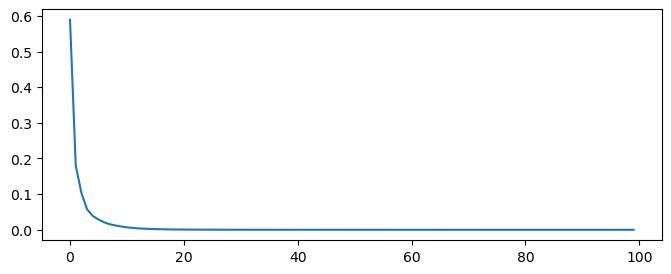
\includegraphics[width=0.5\textwidth]{chapter-2/images/err_0.001.jpg}\\
        \multicolumn{2}{c}{With $\epsilon=10^{-3}$.}\\[0.2cm]
        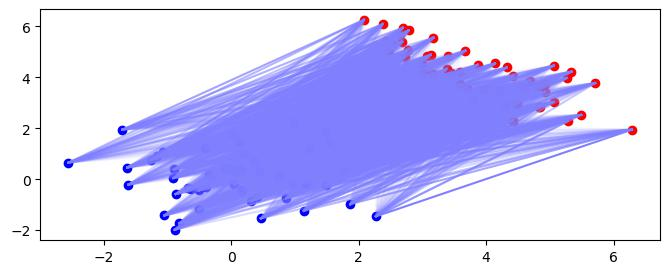
\includegraphics[width=0.5\textwidth]{chapter-2/images/0.1.jpg} & 
        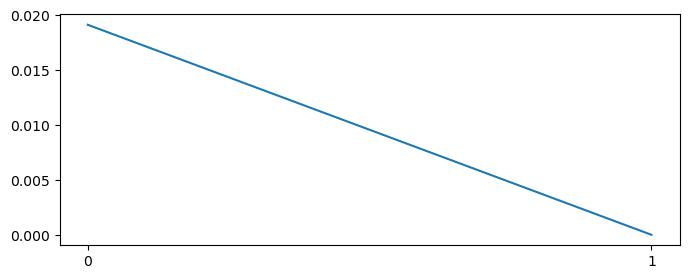
\includegraphics[width=0.5\textwidth]{chapter-2/images/err_0.1.jpg}\\
        \multicolumn{2}{c}{With $\epsilon=10^{-1}$.}\\
    \end{tabular}
    \caption[Illustration of the trade-off of the level of the sparsity of the OT plan and the numerical stability of the Sinkhorn algorithm for solving the entropy-regularized OT formulation.]{The OT plan (left) and the Convergence plot (right) are shown with different coefficients of entropic regularization ($\epsilon$). The non-zero values in the OT plan are shown as edges between the two sets of points (shown in red and blue). The color intensity of an edge represents the value corresponding to the two connecting points. Using $\epsilon=10^{-3}$ results in a sparser transport plan, but the Sinkhorn solver fails to converge even after 100 iterations. With $\epsilon=10^{-1}$, the convergence happens in just 1 iteration, but it results in a dense OT plan.}\label{fig:entr-sparsity}
\end{figure}

Sparser transport plans are preferred as they bring more interpretability in alignments \citep{muzellec17a,swanson-etal-2020-rationalizing} and are suited for budget-constrained mappings \citep{liu2023sparsityconstrained}. Our work proposes a submodular framework to induce sparsity patterns resulting in $K$-sparse solutions that have at most $K(>0)$ non-zero entries. More specifically, we focus on two sparsity patterns: (i) the overall OT plan being $K$-sparse and (ii) each column (or row) of the OT plan being $K$-sparse. While the search space of this constrained optimization is non-convex and non-smooth, we show that our proposed optimization problem is equivalent to the maximization of a weakly submodular function under well-studied matroid constraints. Furthermore, although greedy algorithms providing constant-factor approximation ratios have been studied for maximizing a (weakly) submodular function under matroid constraints, these algorithms often incur significant costs for repeated function calls. To address this, we propose efficient gradient-based greedy algorithms that maintain similar approximation guarantees. We also show that the proposed solver is better in terms of the duality gap when compared to existing approaches that are based on solving an equivalent continuous optimization problem.
\section{Contributions}
The main contributions of this chapter are summarized as follows.
\begin{itemize}%[itemsep=1pt,topsep=0pt]
    \item We first establish an equivalence between the OT formulation and a combinatorial optimization problem involving the support points of the transport plan. We then show that the set function appearing in our combinatorial optimization is weakly submodular when one uses the OT formulation with squared-MMD regularization (MMD-OT in Chapter~\ref{chap:ch1}). This key result is derived based on our proof of strong convexity and smoothness of MMD-OT.
    
    Such an equivalence between an OT problem and a combinatorial optimization may be of independent interest, even beyond the application of inducing sparsity in the transport plan.
    \item We show that the problem of inducing sparsity patterns in the OT plan can be cast as the problem of maximization of a weakly submodular function under matroid constraints. The constraint corresponding to the overall transport plan being $K$-sparse is shown to be equivalent to a Uniform Matroid structure, and the constraint corresponding to each column/row of the plan being $K$-sparse is shown to be equivalent to a Partition Matroid structure.
    \item We propose novel gradient-based greedy algorithms to solve the combinatorial optimization problems corresponding to the two patterns of sparsity constraints on the transport plan discussed above. We also derive the corresponding approximation ratios that resemble the constant-factor approximation ratios of classical greedy algorithms for submodular maximization. 
\item As the problem of finding a sparse transport plan is a non-convex problem, we discuss the efficacy of the proposed solver in terms of the duality gap. The usual approximation results corresponding to greedy maximization of (weakly) submodular functions provide us with lower bounds on the function values. The duality gap analysis provides a more optimistic bound on the performance. The proposed approach obtains a better (lower) duality gap than existing solvers for optimizing the original continuous optimization problem.
\item Finally, we empirically demonstrate the utility of our approach in several applications, including designing a network topology under budget constraints, aligning words in two sentences, and learning a sparse mixture of experts.
\end{itemize}
\section{Preliminaries for the Chapter}\label{sec:sot-prel}
We begin by recalling relevant notations and introducing new ones specific to this chapter. We then also discuss the relevant background materials specific to this chapter.
\paragraph{Notations.} We consider the subspace for the support of the distributions $\mathcal{X}$ as $\mathbb{R}^d$, $d>0$. Let $\hat{s}_m=\sum_{j=1}^m \mathbf{s}_m \delta_{\bx_{1j}}$ and $\hat{t}_n=\sum_{j=1}^n \mathbf{t}_n \delta_{\bx_{2j}}$ be the given empirical/discrete measures. $\bgamma \in \R_+^{m\times n}$ denotes the finitely-parameterized transport plan. For $m \in \mathbb{N}$, $[m] $ denotes the set $  \{1,2,\dots, m\}$. $\bG_{11}\in \R^{m\times m}$ and $\bG_{22}\in \R^{n\times n}$ are the Gram matrices computed over $\{\mathbf{x}_{1j}\}_{j=1}^m$ and $\{\mathbf{x}_{2j}\}_{j=1}^n$, respectively. $\bC\in \R^{m\times n}$ is the cost matrix between $\{\mathbf{x}_{1j}\}_{j=1}^m$ and $\{\mathbf{x}_{2j}\}_{j=1}^n$. The objective for MMD-OT formulation (Chapter~\ref{chap:ch1}) with squared-MMD regularization and finitely-parameterized transport plan is denoted by $\calWF$.


Let $V\coloneqq \{(i,j): i\in[m];\ j\in [n]\}$ represent the index set of an $m\times n$ matrix containing candidate points in the support set of the OT plan. Following the standard terminology, we call $V$ as the ground set. $|\cdot|$ denotes the cardinality of the (set) argument. $F(\cdot)$ is our discrete set function of the support points. $F(a|S)\coloneqq F(S\cup \u)-F(S)$ and is called the marginal gain on adding $a(\in V)$ to $S(\subseteq V)$. We denote the empty (null) set by $\emptyset$. We denote $\alpha\in (0, \infty)$ to denote the submodularity ratio.
Let ${\rm vec}(\mathbf{M})$ denote the row-major vectorization of the matrix $\mathbf{M}$. We use $\mathbf{g}$ vector to denote the gradient of the proposed objective w.r.t. $\bgamma$, and for $a= (i, j)$, $\mathbf{g}_a$ denotes the gradient w.r.t. $\bgamma_{ij}$.
For a non-negative vector $\bz\in\R^d_{+}$, the indices of non-zero entries in $\bz$  are denoted by the set $\Supp(\bz)\coloneqq \{i\in [d]:\bz_i>0\}$. We use small-case $k$ to denote the kernel involved in MMD and $K$ to denote the upper bound on the number of non-sparse entries.
\subsection{Matroid Structure}
Matroids represent a naturally occurring constraint structure in combinatorial optimization. We begin with a formal definition of Matroids and then discuss specific examples which are relevant to this chapter.
\begin{definitionBox}
    \begin{definition}{\textbf{Matroid.}}\\
        Given a finite set $V$ and $\calI\subseteq 2^V$, a set system, $\calM\coloneqq (V, \ \calI)$, is a matroid if\\
        (i) \ \ $\emptyset\in \calI$;\\
        (ii) \ If $A\subseteq B\in \calI$ then $A\in \calI$;\\
        (iii) If $A, B\in \calI$ and $|A|<|B|$, then there is $a \in B\setminus A$ such that $A\cup \u \in \calI$.
    \end{definition}
\end{definitionBox}
Any set system satisfying properties (i) and (ii) is called an \textit{independence system}. The elements of $\calI$ are said to be  \textit{independent} and the elements of $(2^V\setminus \calI)$ are said to be \textit{dependent}. An independence system that additionally satisfies property (iii), also known as Exchangeability, becomes a matroid. Maximal independent sets of a matroid are termed as the \textit{base of a matroid} \citep[Chapter 13]{matroid-korte12}.

It is easy to see that the collection of sets with their cardinalities upper-bounded by $K$ form a matroid. This structure $\mathcal{I}\coloneqq\{A\subseteq V: |A|\leq K\}$ forms a \textbf{Uniform Matroid}. The base of a Uniform Matroid consists of sets that have cardinalities of exactly $K$. 

To see another example, consider sets $P_1, P_2, \ldots, P_n$, which form a partition of $V$, i.e. the union of these disjoint sets gives back $V$. Given the parameters $k_1, \ldots, k_n$, $\mathcal{I}\coloneqq \{A\subseteq V: |A\cap P_y|\leq k_y\ \forall y\in [n]\}$ forms a \textbf{Partition Matroid}. The base of such matroids consists of sets whose intersection with $P_y$ has cardinality exactly $k_y$ for all $y\in [n]$.

\subsection{Submodularity and Weak Submodularity}\label{prelim:subm}
A Submodular function is a discrete set function that exhibits a diminishing returns property, i.e. the marginal gain of adding a new element $\u$ to a set $A$, written as $F(a|A)\coloneqq F(A\cup \u)-F(A)$, diminishes as the set $A$ grows in size.
\begin{definitionBox}
\begin{definition}{\textbf{Submodular Function.}}\label{defn:subm}\newline
A set function $F:2^V\mapsto \R$ is submodular iff $\forall A \subseteq B \subseteq V$ and $a\in V\setminus B$, we have that $F(A\cup \u)-F(A) \geq F(B\cup \u)-F(B), \textup{ i.e. } F(a|A)\geq F(a|B).$
\end{definition}
\end{definitionBox}
As an example, consider a simple set function, $F(S)= \mathbbm{1}_{|S|>0}$. Here, for any $a\in V$, $F(a|\emptyset)> F(a|B),\ \forall \emptyset\subset B \subseteq V$ and $F(a|A)=F(a|B)$ whenever $\emptyset \subset A\subseteq B\subseteq V$ or when $A=B=\emptyset$. Thus, this $F(\cdot)$ is a submodular function. For a detailed review of submodularity and its applications in ML, we refer the interested readers to \citet[Chapter (44)]{matroid} and \cite{Bach2011LearningWS}. Recent approaches of \textit{learning} a submodular function using parametric models can be found in \cite{dsf,sea-nn,de2022neural,extDSF}.

Combinatorial optimization involving a submodular function under different constraint sets is an active area of research. While the minimization of a submodular function relates to the minimization of a convex function and can be solved exactly in polynomial time, the maximization problem is NP-Hard \citep{Bach2011LearningWS}. However, for a non-negative submodular function which is also monotone, i.e. satisfies $F(A)\leq F(B)\ \forall A\subseteq B\subseteq V$, there are efficient approximation algorithms for maximization of such functions over naturally-occurring constraint sets like that of cardinality constraints. Consider a simple iterative greedy algorithm that initializes $S_0\coloneqq \emptyset$ and greedily constructs the sets $S_t \coloneqq  S_{t-1}\cup \ \argmax_{a\in V\setminus S_{t-1}} F(S_{t-1}\cup \u)$ for $t\in [K]$. \cite{DBLP:journals/mp/NemhauserWF78} showed that this greedy algorithm obtains a constant-$(1-1/e)$-factor approximation to the optimal objective for maximizing a submodular function under cardinality constraints, given by $K$. In order to improve the computational performance, stochastic greedy algorithms \citep{mirzasoleiman15a}, also known as lazy greedy algorithms, are popularly used where, at iteration, $t$, the search for the next element is restricted to a stochastically chosen subset of the remaining elements ($V\setminus S_{t-1}$). The corresponding approximation ratio is $(1-1/e-\zeta)$ where $\zeta\in (0, 1)$ is a parameter that inversely affects the size of the stochastically chosen subset of the remaining elements at each $t$.

\paragraph{Weak Submodularity.} \cite{DasKempe18} introduced the notion of weak submodularity governed by a submodularity ratio. For a non-negative monotone function $F(\cdot)$, the submodularity ratio w.r.t. a set $S$ and a parameter $K\geq 1$ is defined as $\alpha_{L, K}(F)\coloneqq \min\limits_{S\subseteq L, A:|A|\leq K, A\cap S=\emptyset}\frac{\sum_{a\in A}F(S\cup \u)-F(S)}{F(S\cup A)-F(S)},$ with $0/0\coloneqq 1$. This ratio is always non-negative. If $\alpha_{L, K}\geq 1, \ \forall L\subseteq V, \forall K\ge 1$, then $F(\cdot)$ is submodular, else $F(\cdot)$ is weakly submodular whenever the ratio is finite. 

Equivalently, a function is said be $\alpha$-weakly submodular for some $\alpha\in (0, 1]$, if $\sum_{a\in A}F(a|S)\geq \alpha. F(A|S)\ \forall S, A\subseteq V$. In our work, to prove a function $F(\cdot)$'s (weak) submodularity, we show that the ratio $\frac{\sum_{a\in A}F(S\cup \u)-F(S)}{F(S\cup A)-F(S)}\in (0, \infty)\ \forall S, A\subseteq V$.

We recall the greedy algorithm discussed above. Starting with $S_0\coloneqq \emptyset$, the greedy algorithm builds the solution set following $S_t \coloneqq  S_{t-1}\cup \ \argmax_{a\in V\setminus S_{t-1}} F(S_{t-1}\cup \u)$.
This algorithm obtains an approximation ratio of $(1-e^{-\alpha})$ for maximizing an $\alpha$-weakly submodular function under cardinality constraints \citep{DasKempe18}. The stochastic greedy algorithm that searches for the next element in a stochastically chosen subset of the remaining elements obtains an approximation ratio of $(1-e^{-\alpha}-\zeta)$ with $\zeta\in (0, 1)$ as the stochasticity parameter that inversely affects the size of the chosen subset \citep{Khanna2017ScalableGF}. Generalizing the cardinality constraints to the case of general matroids, \cite{pmlr-v80-chen18b} have proposed a stochastic greedy algorithm that obtains an approximation ratio of $(1+1/\alpha)^{-2}$ for maximizing a weakly submodular function under matroid constraints.
\subsection{Restricted Strong Concavity and Smoothness}\label{Prel:rsc} 
We discuss a useful property of continuous functions for our analysis of the proposed formulation. Consider a continuously differentiable function $f:\R^N \mapsto \R$. The property of strong concavity and smoothness of $f$ restricted over $(\bx, \ \by)\in\Omega\subseteq \R^N \times \R^N$ is restated from \citet[Definition 3.2]{prajain} as follows. 
\begin{definitionBox}\label{rsm-rsc}
\begin{definition}{\textbf{Restricted Strong Concavity and Smoothness.}}
$$\frac{u_\Omega}{2}\|\by-\bx\|_2^2\leq f(\bx) - f(\by)+\langle\nabla f(\bx), \by-\bx\rangle \leq \frac{U_\Omega}{2}\|\by-\bx\|_2^2,$$
where $u_\Omega$ is called the restricted strong concavity parameter (RSC) and $U_\Omega$ is called the restricted smoothness parameter (RSM) over $\Omega$.
\end{definition}
\end{definitionBox}
With $\Omega$ as $\R^N \times \R^N$, $u_\Omega$ and $U_\Omega$ recover strong concavity and smoothness parameters of $f$, whenever they exist.

Our work involves computing the RSC and RSM parameters of an expression for the objective of MMD-OT as a function of $K$-sparse (vectorized) transport plans.
Thus, we consider $\Omega_K \coloneqq \{ (\bx, \by)\in \R^N\times \R^N~|~ \bx, \by \geq 0; \|\bx\|_0 \leq K; \|\by\|_0 \leq K\}$. We denote the restricted strong concavity (RSC) parameter over $\Omega_K$ as $u_{K}$ and the restricted smoothness (RSM) parameter over $\Omega_K$ as $U_{K}$. An important relation that we use in our work is that when $\hat{K} \leq K$, then $u_{\hat{K}} \geq u_K$ and $U_{\hat{K}} \leq U_K$ which follows by noting that $\Omega_{\hat{K}} \subseteq \Omega_{K}$. We also define $\tilde{\Omega}\coloneqq  \{(\bx,\by)\in \R^N\times \R^N~|~ \|\bx-\by\|_0 \leq 1\}$  with the corresponding restricted smoothness parameter $\tilde{U}_1$.

\section{Literature Review}\label{sec:sot-relw}
\begin{table*}[t]
  \caption[Summarizing the comparison of the proposed Sparse-OT framework with related works.]{Summary of related works and the proposed sparsity-constrained OT formulation.}
  \label{table:sot-relw}
  % \begin{center}
  \centering
  \setlength{\tabcolsep}{0.25em}
  \begin{tabular}{lccc}
    \toprule
     Property & Blondel et al. [2018] & Liu et al. [2023] & \cellcolor{green!10} Proposed\\
     & (SSOT) & (SCOT) & \cellcolor{green!10} (Sparse-OT)\\
    \midrule
    Explicit cardinality constraints & \tikzxmark & \tikzcmark &  \tikzcmark\\
    General sparsity & \tikzcmark & \tikzxmark &  \tikzcmark\\
    Structured sparsity & \tikzxmark & \tikzcmark &  \tikzcmark\\
    With unnormalized measures & \tikzxmark & \tikzxmark &  \tikzcmark\\
    \bottomrule
  \end{tabular}
  % \end{center}
\end{table*}
The OT plan is popularly used in
several applications that involve a distribution-aware alignment between two sets of objects \citep{alvarez18wordEmb,clark2022unified,arase-etal-2023-unbalanced,liu2023sparsityconstrained}. 
\cite{strucOT} motivated the problem of inducing specific structures in the transport plan with a focus on capturing the correlations in the mapping of points which are similar. The authors highlight the need for non-linear cost functions to incorporate such dependencies and propose a submodular cost function for the same. 
Unlike the proposed work, the focus in \cite{strucOT} is not on inducing structured sparsity in the OT plan.


The efforts to induce sparsity in transport plans began with \cite{blondel18a}, who demonstrated that replacing entropic regularization with a squared $\ell_2$-norm or group lasso regularization results in sparser transport plans while maintaining the problem differentiable everywhere. The smoothness of the resulting objective shows computational benefits as well. We will refer to this approach as \textit{SSOT} (smooth and sparse OT). Recent works \citep{wiesel2024sparsityquadraticallyregularizedoptimal,gonzálezsanz2024sparsityquadraticallyregularizedoptimal} have also performed statistical analysis on the support of the sparse transport plans resulting from quadratic regularization. As SSOT does not provide an explicit cardinality control on the level of sparsity, \cite{liu2023sparsityconstrained} proposed sparsity-constrained OT formulation, henceforth termed \textit{SCOT}, with cardinality constraints on each column/row of the OT plan. \cite{liu2023sparsityconstrained} solve a (semi-)dual relaxation of their $\ell_2$-regularized primal formulation using the LBFGS \citep{LBFGS} or ADAM \citep{KingBa15} solvers. These formulations are specific to the Balanced OT variant and do not generalize to Unbalanced OT (Sec.~\ref{bgeqn:uot}).
The need for relaxing the marginal matching constraints in the OT formulation to cater to unnormalized measures \citep{Liero2018,ChizatPSV18} or to provide robustness \citep{Frogner15,jumbot,ROT} led to several Unbalanced OT (UOT) formulations where typically a KL-divergence-based regularization was employed for (softly) enforcing marginal constraints. Recently, \cite{mmd-uot} showcased the efficacy of MMD regularization as an alternative to KL-regularized UOT. We detailed this in Chapter~\ref{chap:ch1} and will refer to their squared-MMD regularized OT formulation with a finitely parameterized transport plan as \textit{MMD-OT} in this chapter. The original UOT formulation (Sec.~\ref{bgeqn:uot}) does not learn structured sparse transport plans with explicit cardinality constraints. We propose a sparsity-constrained OT formulation that builds upon the MMD-OT formulation and generalizes to the Unbalanced OT setting. We compare the proposed approach with related works in Table~\ref{table:sot-relw}.

\section{Proposed Methodology}\label{sec:sot-meth}
We begin with revisiting the squared-MMD regularized OT formulation with a finitely parameterized transport plan from Chapter~\ref{chap:ch1}. Given a cost matrix $\bC$ and a universal kernel $k$ \citep{SriperumbudurFL11}, the MMD-OT formulation is restated as follows.
\begin{equation}\label{eqn:uotmmd}
\begin{array}{l}
\min\limits_{\bgamma\geq \bzero} \ \ \calWF(\bgamma), \ \rm{where} \\
~~\qquad \calWF(\bgamma)\coloneqq \Tr(\bgamma \bC^\top) 
+ \lambda_1{\rm MMD}^2_k(\bgamma\bone,\ \bmu) 
+ \lambda_1{\rm MMD}^2_k(\bgamma^\top\bone,\ \bnu)+ \frac{\lambda_2}{2}\|\bgamma\|^2.
\end{array}
\end{equation}
% \begin{equation}\label{eqn:uotmmd}
% \begin{array}{l}
% \min\limits_{\bgamma\geq \bzero} \ \ \Tr(\bgamma \bC^\top) 
% + \lambda_1{\rm MMD}^2_k(\bgamma\bone,\bmu) + \lambda_1{\rm MMD}^2_k(\bgamma^\top\bone,\bnu)+ \frac{\lambda_2}{2}\|\bgamma\|^2,
% \end{array}
% \end{equation}
Here ${\rm MMD}_k(\bgamma\bone,\ \bmu) = \|\bgamma\bone-\bmu\|_{\bG_{11}}$, ${\rm MMD}_k(\bgamma^\top\bone,\ \bnu) = \|\bgamma^\top\bone-\bnu\|_{\bG_{22}}$ with $\bG_{11}$ and $\bG_{22}$ as the Gram matrices (obtained with kernel $k$) over the source and target samples, respectively. $\Lambda=\{\lambda_1, \lambda_2\}$ is the set of regularization hyperparameters. The regularization hyperparameter $\lambda_1>0$ and we may additionally employ a squared $\ell_2$-norm regularization ($\lambda_2\geq 0$) for computational benefits that would be discussed later in the chapter.

We now propose a formulation for inducing structured sparsity in transport plans. In this regard, we generalize Eq. \ref{eqn:uotmmd} by introducing additional (structured) sparsity constraints on the transport plan as follows:
\begin{equation}\label{eqn:sparse-uotmmd}
\min\limits_{\bgamma\in \calC}\ \calWF({\bgamma}),
\end{equation}
where $\calWF: \R^{m\times n}_{+}\mapsto \R_{+}$ is the function defined in (\ref{eqn:uotmmd}) and $\calC$ denotes a set of sparsity constraints. In this work, we focus on two different sparsity constraints: (i) $\calC$ as $\calC_1\coloneqq \{\bgamma\in\R^{m\times n}_{+}:\|{\rm vec}(\bgamma)\|_0\leq K_1\}$ or (ii) $\calC$ as $\calC_2\coloneqq \{\bgamma\in\R^{m\times n}_{+}:\|\bgamma_j\|_0\leq K_2\ \forall\, j\in[n]\}$, where $\|\cdot\|_0$ denotes the $\ell_0$-norm and $\bgamma_j$ denotes the $j^{\rm{th}}$ column of matrix $\bgamma$. $\calC_2$ can be accordingly modified to incorporate sparsity on each row.
While $\calC_1$ imposes a cardinality constraint on the entire transport plan $\bgamma$, $\calC_2$ imposes the cardinality constraint on each column of $\bgamma$. We highlight that the original MMD-OT formulation is a special case of Problem~\ref{eqn:sparse-uotmmd}, e.g. when $K_1= mn$ or $K_2= m$. 
% \subsection{Problem Formulation}\label{sec:sot-forml} 
\subsection{Reformulation as a Combinatorial Optimization}\label{sec:sot-forml-subm}
The MMD-OT formulation (Eq.~\ref{eqn:uotmmd}) is a smooth and convex problem which can be solved with the accelerated projected gradient descent (APGD) solvers (Refer to Sec.~\ref{comput} in Chapter \ref{chap:ch1}). Despite the convexity of $\calWF$, adding the constraints to enforce sparsity results in Problem~\ref{eqn:sparse-uotmmd} that is non-convex with a non-smooth search space. This motivates us to propose approximation-based solvers for Problem~\ref{eqn:sparse-uotmmd}.

We first note that the solution to the continuous optimization problem in Problem~\ref{eqn:sparse-uotmmd} is the same as the solution to the following continuous optimization problem over discrete sets representing the support of $\bgamma$,
\begin{equation*}
\begin{array}{l}
\max\limits_{S\in V} -\min\limits_{\bgamma:\Supp(\bgamma)\subseteq S,\bgamma\geq \bzero} \calWF({\bgamma}).
\end{array}
\end{equation*}
Adding $\calWF(\bzero)$ makes the inner set function non-negative.
Furthermore, the constraint sets $\calC_1$ or $\calC_2$ essentially restrict the support of the transport plan $\bgamma$ to certain patterns which could be modeled using a matroid structure.
For instance, the set $\calC_1$ may equivalently be represented as a uniform matroid $\calM_1=(V, \ \calI_1)$ where $\calI_1=\{S\subseteq V: |S|\leq K_1\}$. 
Similarly, the set $\calC_2$ may be equivalently modeled using a partition matroid $\calM_2=(V,\ \calI_2)$ where $\calI_2=\{S: S\subseteq V; |S\cap P_j|\leq K_2\, \forall\, j\in [n]\}$ with $P_j=\{(i, j): i\in [m]\}$. Depending on the context, we use $\mathcal{M}$ to denote either $\mathcal{M}_1$, in which case $\mathcal{I}(\mathcal{M})=\mathcal{I}_1$, or $\mathcal{M}_2$, in which case $\mathcal{I}(\mathcal{M})=\mathcal{I}_2$.

With these interesting correspondences, we propose the following combinatorial optimization equivalent to the sparsity-constrained OT problem (\ref{eqn:sparse-uotmmd}).
\begin{definitionBox}
\begin{equation}\label{eqn:reform}
\begin{array}{l}
\max\limits_{S\in \calI(\calM)} F(S), \ \rm{where} \\
~~~\qquad F(S)\coloneqq \calWF(\bzero)-\min\limits_{\bgamma:\Supp(\bgamma)\subseteq S,\bgamma\geq \bzero} \calWF({\bgamma}).
\end{array}
\end{equation}
\end{definitionBox}
This reformulation decouples the original non-convex problem with non-smooth problem search space (Eq.~\ref{eqn:sparse-uotmmd}) into a combinatorial optimization problem whose objective requires solving a convex optimization problem.
For a candidate set $S\in \calI(\calM)$, computing $F(S)$ essentially requires solving the MMD-OT problem (Eq. \ref{eqn:uotmmd}) with the support of $\bgamma$ restricted to set $S$. Since the objective $\calWF(\bgamma)$ is $L$-smooth, (Eq.~\ref{eqn:uotmmd}) can solved using the accelerated projected gradient descent (APGD) method with a fixed step-size of $1/L$ and has a linear convergence rate (Sec.~\ref{comput}).

We now discuss the details for solving Problem~\ref{eqn:reform}. While combinatorial optimization problems could be NP-Hard and may require an exhaustive search, if the corresponding objective function exhibits submodularity, one may devise efficient approximation algorithms (Sec.~\ref{prelim:subm}). To this end, one of our key contributions is our next result, which proves that the set function $F(\cdot)$ is weakly submodular under mild conditions on the kernel function used in $\calWF$. Our proof involves characterization of the function $(-\calWF)$ in terms of the restricted strong concavity (RSC) and restricted smoothness (RSM) parameters (Sec.~\ref{Prel:rsc}) over the restricted domain of $K$-sparse OT plans. From the earlier discussion, we recall that $K=K_1$ when $\mathcal{M}=\mathcal{M}_1$ (overall sparsity) and $K=nK_2$ (column-wise sparsity) when $\mathcal{M}=\mathcal{M}_2$. Let $N=m\times n$. We recall (from Sec.~\ref{Prel:rsc}) the restricted domains we consider as $\Omega_K\coloneqq \{ (\bx, \by)\in \R^N\times \R^N~|~ \bx, \by \geq 0; \|\bx\|_0 \leq K; \|\by\|_0 \leq K\}$ and $\tilde{\Omega}\coloneqq \{ (\bx, \by)\in \R^N\times \R^N~|~ \|\bx-\by\|_0\leq 1 \}$.

\begin{theoremBox}
\begin{restatable}{theorem}{lemmasubm}\label{lemma:subm}
The function $F(\cdot)$ is monotone, non-negative, and $\alpha$-weakly submodular with the submodularity ratio $\alpha\geq \frac{u_{2K}}{\tilde{U}_1}>0$, where $K$ denotes the sparsity level of the transport plan $\bgamma$, whenever the kernel function used in $\calWF$ is universal \citep{SriperumbudurFL11} and bounded. Here, $u_{2K}$ is the RSC parameter of $(-\calWF)$ over $\Omega_{2K}$ and $\tilde{U}_1$ is the RSM parameter of $(-\calWF)$ over $\tilde{\Omega}$.
\end{restatable}
\end{theoremBox}
The proof of Theorem~\ref{lemma:subm} is discussed in Appendix~\ref{app-lemma:subm}. 

Now, leveraging Theorem~\ref{lemma:subm}, we discuss efficient greedy algorithms with attractive approximation guarantees for solving Problem~\ref{eqn:reform} for learning a transport plan with (column-wise) control on the level of sparsity.
\subsection{Learning Sparse Transport Plan}\label{gen-sparse}
We first present the proposed approach for learning transport plans with cardinality constraints on the number of non-zero (non-sparse) elements.
A sparser transport plan improves interpretability in the resulting alignments \citep{swanson-etal-2020-rationalizing} and can be useful in applications such as designing network topology with constraints on the number of edges \citep{ijcai2023p679}, aligning words in two sentences \citep{arase-etal-2023-unbalanced}, etc. 

For learning cardinality-constrained sparse transport plans, we propose Problem~\ref{eqn:reform} with $\calM = \calM_1$, i.e., 
\begin{equation}\label{eqn:gensparse}
\max\limits_{S\in \calI_1} F(S). 
\end{equation}
The solution to this optimization problem will have a maximum of $K=K_1$ non-zero entries. We term this formulation as \textbf{General-SparseOT} to indicate the general (non-structural) sparsity constraints involved. 

We now discuss solving the General-SparseOT formulation.
Problem~\ref{eqn:gensparse} involves the maximization of a set function under cardinality constraints. From Theorem~\ref{lemma:subm}, we know that the function involved is monotone, non-negative and $\alpha$-weakly submodular and consequently, the classical greedy algorithm \citep{DasKempe18}, discussed in Sec.~\ref{prelim:subm}, can be employed to solve the problem with a constant-factor approximation ratio of $(1-e^{-\alpha})$ \citep{DasKempe18}.
This greedy algorithm starts with an empty set $S_0 \coloneqq \emptyset$, and at each iteration $t$, it finds an element $a\in V\setminus S_{t-1}$ such that the marginal gain $F(a|S_{t-1})$ is maximized.
We detail the greedy algorithm for solving Problem~\ref{eqn:gensparse} in the Appendix (Algorithm~\ref{alg:gensparseOT_greedy}). The function $F(\cdot)$, however, requires solving a number of instances of the MMD-OT optimization problem for evaluating the marginal gain corresponding to all the unselected elements (in step 3 of Algorithm~\ref{alg:gensparseOT_greedy}), in each outer iteration. This accounts for a total $\left(mnK-\frac{K(K-1)}{2}\right)$ calls to the MMD-OT optimization problem. A more computationally efficient approach would be the gradient-based greedy algorithm similar to \citet[Algorithm (2)]{gurumoorthy19a}. This approach chooses the next element to be added to the support set greedily based on the gradient vector, $(-\nabla \calWF(\cdot))$ (Eq.~\ref{eqn:gradient}), instead of the marginal gains. We detail this algorithm in the Appendix (Algorithm~\ref{alg:gensparseOT_dash}). We can see that this reduces the overall number of calls to the MMD-OT optimization module from $\left(mnK-\frac{K(K-1)}{2}\right)$ to $K$ which is a significant drop when $mn$ is large (as is the case in large-scale ML applications), and $K$ is small. 

Improvising these algorithms, we propose our gradient-based greedy algorithm by incorporating the concepts from stochastic greedy algorithms \citep{mirzasoleiman15a,Khanna2017ScalableGF}. This includes solving the MMD-OT problem (\ref{eqn:uotmmd}) for a given support set $S$ and using its solution $\bgamma$ to compute the gradient $(-\nabla\calWF(\bgamma_{S_{t-1}}))$ only for a randomly chosen subset of elements $R_t$ where $t>0$. We present the proposed approach in Algorithm~\ref{alg:stoch-dash}. We can see that Algorithm~\ref{alg:stoch-dash} requires solving the MMD-OT problem (\ref{eqn:uotmmd}) of size $|t|$ only once in each iteration $t$. Step~3 in Algorithm~\ref{alg:stoch-dash} corresponds to stochastic selection of the candidate set $R_t$ at iteration $t$ \citep{mirzasoleiman15a,Khanna2017ScalableGF}. 

\begin{algorithm}[t]
\caption[Proposed algorithm for learning sparse transport plans]{Proposed algorithm for learning sparse transport plans}
\begin{algorithmic}[1]
\Require  $\lambda_1, \lambda_2, \bmu, \bnu, \bC, \bG_{11}, \bG_{22}$, sparsity level $K_1$, $\zeta$.
\State $S_0=\emptyset, \bgamma_{S_0} = \bzero$ and $\mathbf{g} = -\nabla \calWF(\bgamma_{S_0})$.
\For{$t=1,\ldots,K_1$}
\State $R_t\leftarrow$ a random subset of $V\setminus S_{t-1}$ with  $mnK_1^{-1}\log(1/\zeta)$ elements 
\State $a \in \argmax_{e\in R_t}{\mathbf{g}_e}$ (ties broken arbitrarily)
\State $S_t = S_{t-1}\cup \u$
\State $\bgamma_{S_t} = \argmin_{\bgamma:\Supp(\bgamma)\subseteq S_t, \bgamma\ge \bzero}{\calWF(\bgamma)}$ %NOTE: argmin is CORRECT. NOT argmax.
\State $\mathbf{g}= -\nabla \calWF(\bgamma_{S_t})$
\EndFor
\State \textbf{return} $S_{K_1}, \bgamma_{S_{K_1}}$
\end{algorithmic}\label{alg:stoch-dash}
\end{algorithm}
 
Compared to the non-stochastic gradient-based greedy approach (Algorithm~\ref{alg:gensparseOT_dash}), Algorithm~\ref{alg:stoch-dash} is more efficient as the gradient is computed only for a subset of the remaining elements.
With $S_K$ as the $K$-sparse solution returned by our algorithm and $S^*$ as the optimal solution for the problem, we present the approximation guarantee of Algorithm~\ref{alg:stoch-dash} for solving Problem~\ref{eqn:gensparse}. 
\begin{lemmaBox}
\begin{restatable}{lemma}{lemmastochdash}\label{lemma:stoch-dash}
Let $\{S_K,\bgamma_{S_K}\}$ be the output returned by the proposed Algorithm~\ref{alg:stoch-dash} for sparsity level $K$. Let $S^{*}$ be an optimal solution of Problem~(\ref{eqn:gensparse}). 
Then, $\mathbb{E}[F(S_K)] \geq (1- e^{-u_{2K}/\tilde{U}_1}-\zeta) F(S^{*})$, where $u_{2K}$ is the RSC parameter of $(-\calWF)$ over $\Omega_{2K}$ and $\tilde{U}_1$ is the RSM parameter of $(-\calWF)$ over $\tilde{\Omega}$.
\end{restatable}
\end{lemmaBox}
The proof of Lemma~\ref{lemma:stoch-dash} is discussed in Appendix~\ref{app-lemma:stoch-dash}.

\subsection{Learning Column-wise Sparse Transport Plan}\label{subsec:partitionmatroid}
We next discuss learning structured sparse OT plans. We present the proposed approach for learning the transport plan $\bgamma$ with cardinality constraints on the number of non-zero (non-sparse) elements in each column of the transport plan. The same approach can also be applied to get transport plans with cardinality constraints on the number of non-zero (non-sparse) elements in each row. A column-wise or row-wise sparse transport plan is especially useful when solving a budget-constraint mapping problem like the one that occurs in mapping inputs to expert neural networks in a sparse mixture of experts model \citep{liu2023sparsityconstrained}. 

To this end, we propose solving Problem~\ref{eqn:reform} with $\calM = \calM_2$, i.e., 
\begin{equation}\label{eqn:colsparse}
\max\limits_{S\in \calI_2} F(S).
\end{equation}
The constraint here is that of a partition matroid which ensures that Problem~\ref{eqn:colsparse} learns a transport plan with each column having at most $K_2$ non-sparse entries. We term this formulation as \textbf{Column-SparseOT}. The total number of non-sparse entries in the learned transport plan $\bgamma$ is $K=nK_2$. 

We now discuss solving the Column-SparseOT formulation. We first note that Algorithm~\ref{alg:stoch-dash} cannot be directly employed for solving Problem~\ref{eqn:colsparse} as its greedy selection does not respect the partition matroid constraint. Hence, we consider the residual randomized greedy algorithm for maximizing weakly submodular functions under the matroid constraints \citep{pmlr-v80-chen18b}. This algorithm presented in the Appendix (Algorithm~\ref{alg:matroid}) provides a $(1+1/\alpha)^{-2}$ approximation ratio for $\alpha$-weakly submodular maximization subject to a matroid constraint. However, this would again incur a higher computational cost as it requires solving multiple MMD-OT instances in each iteration for evaluating the function $F(\cdot)$. Hence, we propose a novel gradient-based randomized greedy algorithm, Algorithm~\ref{alg:colsparseOT_dash}, for maximizing weakly submodular functions subject to matroid constraints.

At each iteration $t$, Algorithm~\ref{alg:colsparseOT_dash} selects a uniformly random element from the best maximal independent set (base) of $\calM_2/S_{t-1}$. 
Here, $\calM_2/S \coloneqq \left(V\setminus S, \calI_{\calM_2/S}\right)$ denotes the contraction of $\calM_2$ by $S$, which is a matroid on $V\setminus S$ consisting of independent sets $\calI_{\calM_2/S} \coloneqq \{I \subseteq V\setminus S: I \cup S \in \calI \}$. 
Further, the gradient $\nabla \calWF(\bgamma_{S_{t}})$ is computed corresponding to the elements in $\{a: a\in \calI_{\calM_2/S_{t-1}}\}$. 
The solution $\bgamma_{S}$ in step~6 is obtained using the accelerated projected gradient descent (APGD)  algorithm. It should be noted that step~3 of Algorithm~\ref{alg:colsparseOT_dash} may not require a search over all possible maximal independent sets of $\calM_2/S_{t-1}$. For partition matroids, step~3 essentially involves selecting the Top-$(K_2-|S\cap P_j|)$ elements from each column $j$ based on the largest (thresholded) gradient values from the set $P_j\setminus S_{t-1}$ for each column $j$.
%column $j$.
The approximation guarantee provided by the proposed Algorithm~\ref{alg:colsparseOT_dash} is as follows. 
\begin{lemmaBox}
\begin{restatable}{lemma}{lemmastrucdash}\label{lemma:struc-dash}
Let $\{S_K,\bgamma_{S_K}\}$ be the output returned by the proposed Algorithm~\ref{alg:colsparseOT_dash} for sparsity level $K=nK_2$. Let $S^{*}$ be an optimal solution of Problem~(\ref{eqn:colsparse}). Then, 
$\mathbb{E}[F(S_{K})]\geq F(S^*)\left(1+\tilde{U}_1/u_{2K}\right)^{-2}$, where $u_{2K}$ is the RSC parameter of $(-\calWF)$ over $\Omega_{2K}$ and $\tilde{U}_1$ is the RSM parameter of $(-\calWF)$ over $\tilde{\Omega}$.
\end{restatable}
\end{lemmaBox}
Appendix~\ref{app-lemma:struc-dash} discusses the proof for Lemma~\ref{lemma:struc-dash}.
\begin{algorithm}[t]
\caption[Proposed algorithm for learning column-wise sparse transport plans]{Proposed algorithm for learning column-wise sparse transport plans} \label{alg:colsparseOT_dash}
\begin{algorithmic}[1]
\Require  $\lambda_1, \lambda_2, \bmu, \bnu, \bC, \bG_{11}, \bG_{22}$, per column sparsity level $K_2$.
\State $S_0=\emptyset, \bgamma_{S_0} = \bzero, K=nK_2,\mathbf{g} = -\nabla \calWF(\bgamma_{S_0})$.
\For{$t=1,\ldots,K$}
\State $M_t\leftarrow$ a maximal independent set of $\calM_2/S_{t-1}$ maximizing $\sum_{a\in M_t}\max(0,\bg_a)$ (ties broken arbitrarily)
\State $a\leftarrow$ a uniformly random element from $M_t$
\State $S_t = S_{t-1}\cup \u$
\State $\bgamma_{S_t} = \argmin_{\bgamma:\Supp(\bgamma)\in S_t,\bgamma\ge \bzero}{\calWF(\bgamma)}$ 
\State $\mathbf{g} = -\nabla \calWF(\bgamma_{S_t})$

\EndFor
\State \textbf{return} $S_{K}, \bgamma_{S_{K}}$
\end{algorithmic}
\end{algorithm}

\subsection{Computational Aspects}
\paragraph{On Solving the MMD-OT Instances.}\label{app:solver}
We begin by discussing how to adapt the solver proposed in Chapter~\ref{chap:ch1} to solve the MMD-OT instances appearing in the proposed Algorithm~\ref{alg:stoch-dash} and \ref{alg:colsparseOT_dash}. When $S$ is the same as $V$ i.e. with no constraints on the support, the objective of MMD-OT optimization appearing in step~6 of Algorithms~\ref{alg:stoch-dash} and \ref{alg:colsparseOT_dash} can be written as follows.
\begin{equation}
\begin{array}{ll}
\calWF(\bgamma)\coloneqq  &\sum\limits_{(i,j)\in V} \big[ \bC_{ij}\bgamma_{ij} + \frac{\lambda_2}{2}\bgamma_{ij}^2 + \lambda_1 \bgamma_{ij} \big( \sum\limits_{(p,q)\in T} \bgamma_{pq} (\bG_{11})_{ip} - 2(\bG_{11}\bmu \bone_{n}^{\top})_{ij} \big) \\
&+ \lambda_1 \bgamma_{ij} \big( \sum\limits_{(p,q)\in T} \bgamma_{pq}(\bG_{22})_{qj} - 2 (\bone_m\bnu ^\top \bG_{22})_{ij} \big) \big]+\lambda_1(\|\bmu\|^2_{\bG_{11}} + \|\bnu\|^2_{\bG_{22}}).
\end{array}
\end{equation}
In Chapter~\ref{chap:ch1}, this objective was shown to be $L$-smooth and subsequently accelerated projected gradient descent (APGD) algorithm with step-size $1/L$ was employed to solve the optimization with a linear convergence guarantee.

With the constraint set $S\subset V$, $\bgamma_{ij}$ (and $\bgamma_{pq}$ terms) can be set to zero for all $(i,j)\in (V\setminus S)$ and all $(p,q)\in (V\setminus S)$. Consequently, the optimization problem only involves $\bgamma_{ij}$ for $(i,j)\in S$. We denote this variable as $\bgamma_S$ in the following:
$$\min_{\bgamma:\Supp(\bgamma)\subseteq S, \bgamma \geq 0}\ \calWF(\bgamma) \coloneqq \min_{\bgamma_S \geq 0}\ \calWF(\bgamma_S), \ \ \textup{where} $$ 
\begin{equation}
\begin{array}{ll}
\calWF(\bgamma_S)\coloneqq  &\sum\limits_{(i,j)\in S} \big[ \bC_{ij}\bgamma_{ij} + \frac{\lambda_2}{2}\bgamma_{ij}^2 + \lambda_1 \bgamma_{ij} \big( \sum\limits_{(p,q)\in S} \bgamma_{pq} (\bG_{11})_{ip} - 2(\bG_{11}\bmu \bone_{n}^{\top})_{ij} \big)\\
&+ \lambda_1 \bgamma_{ij} \big( \sum\limits_{(p,q)\in S} \bgamma_{pq}(\bG_{22})_{qj} - 2 (\bone_m\bnu ^\top \bG_{22})_{ij} \big) \big] + \lambda_1(\|\bmu\|^2_{\bG_{11}} + \|\bnu\|^2_{\bG_{22}}).
\end{array}
\end{equation}
This simplified objective still maintains smoothness as a function of $\bgamma_S$ which has non-zero entries only for the support in $S$. Hence, the optimization problem appearing in step 6 of the algorithms can again be done using the APGD algorithm.

\paragraph{Gradient Computation.} The gradient $\nabla \calWF(\bgamma)$ is employed in steps 7 of both the proposed Algorithms~\ref{alg:stoch-dash}~\&~\ref{alg:colsparseOT_dash}. 
The partial gradient $\frac{\partial \calWF(\bgamma)}{\partial \bgamma_{ij}}$ is as follows:
\begin{align}\label{eqn:gradient}
 \bC_{ij} + 2\lambda_1 \left((\bG_{11})_i^\top (\bgamma \bone_n) +  (\bone_m^\top\bgamma)(\bG_{22})_j\right) - 2\lambda_1 \Big((\bG_{11})_i^\top \bmu
+ \bnu^\top (\bG_{22})_j\Big) + \lambda_2 \bgamma_{ij}.
\end{align}

In (\ref{eqn:gradient}), we observe two things (a) the last term $(\bG_{11})_i^\top \bmu + \bnu^\top (\bG_{22})_j$ is independent of $\bgamma$ and can be precomputed, and 
(b) the terms involving the full matrix $\bgamma$ decouple in $i$ and $j$. 
We leverage this structure for computing $\nabla \calWF(\bgamma)$ efficiently. 

\paragraph{Computational Cost.} We now discuss the per-iteration computational cost of both the proposed algorithms. For a given support set $S$, both Algorithms~\ref{alg:stoch-dash}~\&~\ref{alg:colsparseOT_dash} involve solving the corresponding MMD-OT problem to obtain the solution $\bgamma_S$. Let $R\subseteq V\setminus S$ be the set on which the gradient needs to be computed. The set $S$ is updated via greedy selection as $S_t\leftarrow S_{t-1}\cup \u$, where $a\in R_t$ is the chosen element in the iteration $t$. The per-iteration cost of both the algorithms is $O(N+T\cdot M)$, where $N$ is the cost of computing the gradient of candidate elements, $T$ is the maximum iterations used for solving MMD-OT using APGD, and $M$ is the gradient cost in every APGD iteration. The above expression does not include the one-time cost of computing matrices $\bC,\bG_{11},\bG_{22}$ and vectors $\bG_{11}\bmu,\bG_{22}\bnu$. 

Let $I_S=\{i\in [m]:(i,j)\in S\}$, $J_S=\{j\in [n]:(i,j)\in S\}$, $I_R=\{i\in [m]:(i,j)\in R\}$, and $J_R=\{j\in [n]:(i,j)\in R\}$. 
Then, $M=O(|I_S|^2 + |J_S|^2 + |S|)$ and $N=O(|I_S||I_R| + |J_S||J_R| + |S| + |R|)$. For both the algorithms, $1\leq|I_S|,|I_R|\leq m$ and $1\leq|J_S|,|J_R|\leq n$, where the  value of these terms depend on $S$ and $R$. For Algorithm~\ref{alg:stoch-dash}, $|R|=mnK^{-1}\log(1/\zeta)$ and for Algorithm~\ref{alg:colsparseOT_dash} with the matroid constraint, $2\leq |R|\leq mn$.

\paragraph{Stopping Criteria.} For applications where a budget constraint $K$ is pre-specified, our algorithms involve iterating up to $K$, greedily building the optimal support set $S$ and the corresponding transport plan $\bgamma_S$ supported over $S$. However, when dealing with general sparsity constraints, often, $K$ is not known beforehand, and one would want to choose stopping criteria adaptively. The classical greedy algorithms choose to iterate as long as there is a strictly positive marginal gain, i.e. as long as $F(a|S_{t-1})>0$ where $a\in \argmax_{e\in V\setminus S_{t-1}}\ F(e|S_{t-1})$. As our algorithms are gradient-based greedy algorithms, we discuss equivalent criteria in terms of the gradients. Using the properties of $F(\cdot)$ discussed in the previous section, one can show that,
$F(S_{t-1}\cup \u) - F(S_{t-1})\leq \frac{1}{2u_{(|S_{t-1}|+1)}}\left(\mathbf{g}_a^+(\bgamma_{S_{t-1}})\right)^2,$
where $\mathbf{g}_a^+(\cdot)= \max\{-(\nabla \calWF(\cdot))_a,\ 0\}.$
The proof of Lemma~\ref{lemma2.2} in the Appendix covers this result as a special case.
The above inequality along with the monotonicity property of $F(\cdot)$ gives us that $-(\nabla \calWF(\cdot))_a\leq 0$ implies $F(S_{t-1}\cup \u) - F(S_{t-1})=0$, i.e. no marginal gain on adding $\u$. Thus, for applications where $K$ is not satisfied, we keep the iterations in our algorithms as long as $(\nabla \calWF(\cdot))_a\leq 0$.
\subsection{Computing the Duality Gap}
In the previous sections, we established connections to discrete submodular maximization, proposed gradient-based greedy algorithms, and derived corresponding approximation guarantees in Lemmas~\ref{lemma:stoch-dash} and \ref{lemma:struc-dash}. In this section, we contrast this approach with a continuous-optimization-based approximate solver to Problem~\ref{eqn:sparse-uotmmd}. To this end, in Lemma~\ref{lemma:dual}, we present the dual of Problem~\ref{eqn:sparse-uotmmd}. While only weak duality holds due to the problem being non-convex, the duality gap analysis may still provide insights into the closeness to the optimal objective.
\begin{lemmaBox}
\begin{restatable}{lemma}{lemmadual}\label{lemma:dual}
    Problem \ref{eqn:sparse-uotmmd} with $\calC=\calC_2$ and $\lambda_2>0$ may equivalently be written as: 
    \begin{equation}\label{eqn:primal}
    \begin{array}{l}
        \min\limits_{\bgamma\geq \bzero} P(\bgamma)\big(\coloneqq  \langle\mathbf{C},\bgamma\rangle + \sum_{j=1}^n \Theta(\bgamma_j) + \lambda_1(\|\bgamma\bone-\bmu\|_{\bG_{11}}^2+\|\bgamma^\top\bone-\bnu\|_{\bG_{22}}^2)\big),
    \end{array}
    \end{equation}
    where $\bgamma_j$ denotes the $j^\textup{th}$ column of $\bgamma$, $\Theta(\bgamma_j)=\frac{\lambda_2}{2}\|\bgamma_j\|^2 + \delta_{B_{K_2}}(\bgamma_j)$ and $B_{K_2} = \{\bz\in \R_{+}^m:\|\bz\|_0\leq K_2\}$. Here, $\delta_{B}$ is the indicator function of a set $B$ such that $\delta_{B}(\bz)=0$ if $\bz\in B$, and $\delta_{B}(\bz)=\infty$ otherwise. The following is a convex (weak) dual of the primal (\ref{eqn:primal}):
    \begin{equation}\label{eqn:dual}
    \begin{array}{l}
        \max\limits_{\balpha\in\R^m,\bbeta\in\R^n} D(\balpha,\bbeta) \big(\coloneqq \langle\balpha,\bmu\rangle + \langle\bbeta,\bnu\rangle - \frac{1}{4\lambda_1}\balpha^\top \bG_{11}^{-1}\balpha\\
        \qquad \qquad \qquad \qquad \qquad -\frac{1}{4\lambda_1} \bbeta^\top \bG_{22}^{-1}\bbeta -\sum_{j=1}^n \Theta^*(\balpha+\bbeta_j\bone - \bC_j)\big),
    \end{array}
    \end{equation}
    where $\bC_j$ denote the $j^\textup{th}$ column of $\bC$ and
    \begin{equation}\label{eqn:conjugate}
    \Theta^{*}(\bw) = \max_{\bz\in B_{K_2}} \langle\bw,\bz\rangle - \frac{\lambda_2}{2}\|\bz\|^2 .
    \end{equation}
\end{restatable}
\end{lemmaBox}
Lemma~\ref{lemma:dual} uses Lagrangian duality where $\balpha$ and $\bbeta$ are the Lagrangian parameters corresponding to $\bgamma\bone-\bmu =\bp$ and $\bgamma^\top\bone-\bnu =\bq$ constraints, respectively, where $\bp$ and $\bq$ are auxiliary variables. To compute $\Theta^*(\bw)$, consider the permutation $\pi$ on $[m]$ such that $\bw_{\pi(i)} \geq \bw_{\pi(i+1)}$ for $1\leq i < m$. The solution is given by $\bz_{\pi(i)} =\begin{cases}
    \max\left(0, \frac{\bw_{\pi(i)}}{\lambda_2} \right) & i \in [K_2]\\
    0 & \textup{Otherwise}.
\end{cases}$, and $\Theta^{*}(\bw)=\frac{1}{2\lambda_2}\sum_{i=1}^{K_2} (\max(0,\bw_{\pi(i)}))^2$ \citep{liu2023sparsityconstrained}. 

For a feasible primal-dual pair $\{\bgamma_S,(\balpha_S,\bbeta_S)\}$ corresponding to (\ref{eqn:primal}) and (\ref{eqn:dual}), 
$\Delta(\bgamma_S,\balpha_S,\bbeta_S) = P(\bgamma_S)-D(\balpha_S,\bbeta_S)$ is the associated duality gap. Computing $\Delta(\bgamma_S,\balpha_S,\bbeta_S)$ requires computing the dual candidate $(\balpha_S,\bbeta_S)$ for the given primal candidate $\{\bgamma_S\}$, which leads to our next result. 
\begin{lemmaBox}
\begin{restatable}{proposition}{propdualitygap}\label{prop:dualitygap}
    Let $\bgamma_S$ be a feasible primal candidate for (\ref{eqn:primal}), e.g., obtained from Algorithm~\ref{alg:colsparseOT_dash} as (\ref{eqn:primal}) and (\ref{eqn:colsparse}) are equivalent problems. Then, the dual candidates $(\balpha_S,\bbeta_S)$ corresponding to $\bgamma_S$ are $\balpha_S = 2\lambda_1\bG_{11}(\bmu-\bgamma\bone)$ and $\bbeta_S = 2\lambda_1\bG_{22}(\bnu-\bgamma^\top\bone)$.
\end{restatable}
\end{lemmaBox}
Proposition~\ref{prop:dualitygap} provides concrete expressions for computing the duality gap $\Delta$. While weak duality only guarantees $\Delta\geq 0$, computing $\Delta$ may still provide an estimate of how far a candidate solution could be from optimality in terms of the optimal objective values.

\noindent We present the proofs of Lemma~\ref{lemma:dual} and Proposition~\ref{prop:dualitygap} in Appendix~\ref{app:dual}.
\section{Experimental Results}\label{sec:sot-expt}
We empirically evaluate the proposed approach in various downstream ML applications. Experiments related to inducing overall sparsity in the transport plans are presented in Sec.~\ref{gensparseexp} and~\ref{exp:word-alignment}, while those related to inducing column-wise sparsity are presented in Sec.~\ref{colsparseexp}. 
Additional experimental details and more results are presented in Appendix \ref{app:exp}. The codes to reproduce all experiments are open-sourced at \texttt{https://github.com/Piyushi-0/Sparse-OT}.

\subsection{Designing Topology}\label{gensparseexp}
We begin with an application of the sparsity constraints on the overall OT plan. 
Sparse process flexibility design (SPFD) aims to design a network topology that could handle (unpredictable) demands of $n$ products by matching them to the supplies from  $m$ plants. Nodes correspond to the locations of supply and demand, and designing a network topology requires adding edges between these nodes. These edges facilitate the flow of goods, and it is often desired to design a network topology with a budget constraint on the number of edges. A recent work \citep{ijcai2023p679} models SPFD as an OT problem. While the supplies are predefined and can be modeled as $\bmu\in [0, \infty)^m$, the demands are unpredictable and follow a given distribution $\nu$. Hence, a set of demand vectors $\{(\bnu)_y\}_{y=1}^z$ are sampled from $\nu$, i.e., $(\bnu)_y\in [0, \infty)^n \sim \nu \ \forall y\in [z]$ for a pre-defined $z>0$. With a matrix $\mathbf{P}\in \R^{m\times n}$ denoting profits and $l$ as the total number of edges allowed in the network topology,
\citet[Eq. (3)]{ijcai2023p679} formulates the SPFD problem as follows.
\begin{equation}\label{eqn:spfd}
\max\limits_{ \{ \bgamma_y\in \Gamma(\bmu, (\bnu)_y)\}_{y=1}^z}\frac{1}{z}\sum_{y=1}^z\langle\mathbf{P}, \bgamma_y\rangle,
\ \textup{s.t. }\left\|\sum_{y=1}^z \bgamma_y\right\|_0\leq l.
\end{equation}
Here $\mathbf{P}$ acts as the negative of the cost matrix involved in an OT formulation, and $\Gamma(\bmu, (\bnu)_y)$ denotes the set of feasible OT plans. One could have $\Gamma(\bmu, (\bnu)_y)=\{\bgamma~|~\bgamma\ge \bzero, \bgamma \bone = \bmu, \bgamma^\top \bone = (\bnu)_y\}$ to model the Balanced OT setup.

On obtaining the solutions $\{\bgamma_y\}_{y=1}^z$, an aggregate solution $\bgamma=\frac{1}{z}\sum_{y=1}^z\bgamma_y$ is computed. The top-$l$ edges are chosen from $\bgamma$ for obtaining the budget-constrained network topology given by $\rm{top}_l(\bgamma)$. The profit obtained by the solution is computed as $\langle \mathbf{P}, \rm{top}_l(\bgamma) \rangle$.

\paragraph{Group-Sparse OT (GSOT) Approach.} \citet{ijcai2023p679} perform a convex relaxation of the $\ell_0$-norm constraint in Eq.~\ref{eqn:spfd} with an $\ell_1$-norm regularizer and solve the resulting problem using an ADMM algorithm \citep{admm}. The profits are computed using the resulting OT plans.

\paragraph{Proposed Reformulation.} We observe that the SPFD problem can be equivalently modeled as instances of General-SparseOT Problem~\ref{gen-sparse}. This observation follows from noting the triangular inequality property of the $\ell_0$ norm. If one solves the original SPFD problem~\ref{eqn:spfd} with constraints as $\|\bgamma_y\|_0\leq \frac{l}{z}\ \forall y\in [z]$, this would lead to $z$ instances of General-SparseOT (Problem~\ref{gen-sparse}). Hence, we propose solving the following independent instances of the General-SparseOT problem to solve SPFD.
\begin{equation}\label{eqn:proposed_spfd}
\frac{1}{z}\sum_{y=1}^z\ \max\limits_{\bgamma_y\in \Gamma(\bmu, (\bnu)_y)}\langle\mathbf{P}, \bgamma_y\rangle,\ \textup{s.t. }\|\bgamma_y\|_0\leq \frac{l}{z} \ \forall y\in[z].
\end{equation}
We solve these instances using the proposed Algorithm~\ref{alg:stoch-dash} and compute the profit with the resulting OT plans.

\paragraph{Experimental Setup.} We generate the source and target data samples with $m=n=100$ and $z=20$ using the data generation process described in \citet{ijcai2023p679}. 
We compare the profit generated by the proposed approach and by GSOT \citep{liu2023sparsityconstrained}.
The validation details to choose the best hyperparameters are given in Appendix~\ref{app:spfd}. We evaluate the performance of the proposed approach on varying the stochasticity parameter $\zeta$ in Algorithm~\ref{alg:stoch-dash}. 

\paragraph{Results.}
In Table~\ref{table-top}, we report the expected profit (averaged across five random trials) obtained by both the approaches with $l=\{100,175,250\}$, following the guidelines of choosing $l$ from the range $\max\{m, n\}$ to $\rm{round}(2.5\max\{m, n\})$.
The proposed approach achieves a 10 times higher profit than GSOT showing its efficacy in the SPFD application. Our approach is also computationally more efficient as shown in Table~\ref{table: Time T1}.

\begin{table}[t]
\caption[Evaluation of proposed Sparse-OT framework for the task of designing a budget-constrained network topology.]{Expected profit (higher is better) for the experiment on designing topology with varying network size constraint $l$. The proposed approach involves solving our General-SparseOT formulation (\ref{eqn:gensparse}) with Algorithm~\ref{alg:stoch-dash} and the stochasticity parameter $\zeta$. The results are averaged over five random trials. We observe that our approach outperforms the GSOT baseline. Our approach is also computationally more efficient as shown in Table~\ref{table: Time T1}.}
\label{table-top}
% \vskip 0.15in
\centering
\setlength{\tabcolsep}{4pt}
\begin{tabular}{lccc}
\toprule
Method & $l=100$ & $l=175$ & $l=250$\\
\midrule
    Group-Sparse OT (GSOT) \citep{ijcai2023p679} & {0.014} & {0.031} & {0.044} \\
    \rowcolor{green!10}
    Proposed ($\zeta= 10^{-2}$) & {$0.166$} & {$ 0.224$} & {$ \mathbf{0.293}$}\\
    \rowcolor{green!10}
    Proposed ($\zeta= 10^{-3}$) & {$\mathbf{0.167}$} & {$ 0.238$} & {$0.286$}\\
    \rowcolor{green!10}
    Proposed ($\zeta= 10^{-4}$) & {$0.147$} & {$\mathbf{0.240}$} & {$0.274$}\\
\bottomrule
\end{tabular}
% \vskip -0.1in
\end{table}


\subsection{Monolingual Word Alignment}\label{exp:word-alignment}
Aligning words in a (monolingual) sentence pair is an important sub-task in various natural language processing applications such as question answering, paraphrase identification, sentence fusion, and textual entailment recognition, to name a few \citep{maccartney08,yao13,feldman19,brook21}. Recently, \citet{arase-etal-2023-unbalanced} proposed solving an OT problem between uniform distributions over the set of word embeddings corresponding to the two sentences. \citet{arase-etal-2023-unbalanced} showed that different variants of OT, like the Balanced OT, Partial OT, and Unbalanced OT, outperform the state-of-the-art deep-learning-based techniques \citep{JaliliSabet2020SimAlignHQ} for this task.

\begin{figure}[t]
\centering{
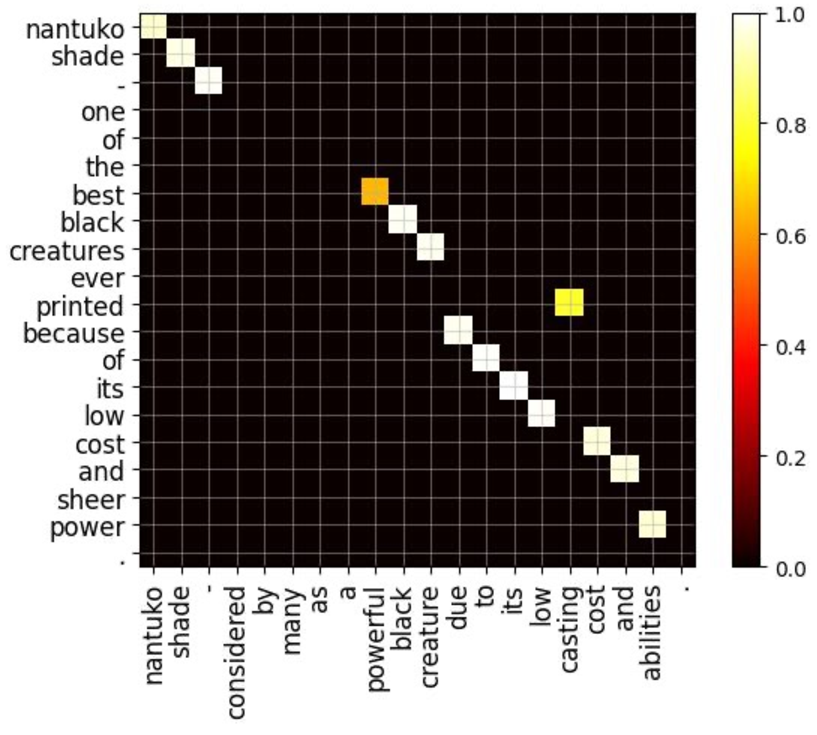
\includegraphics[scale=0.6]{chapter-2/images/proposed-wiki.pdf}
    \caption[Visualizing the alignments of words in a sentence-pair learned by the proposed Sparse-OT framework.]{Example of a word alignment matrix obtained by the OT plan learned with our General-SparseOT formulation.  Words without a semantic counterpart are left unaligned and form \textit{null} alignments.
    }
    \label{App-waln}}
\end{figure}

As words in a sentence may lack semantic counterparts in another sentence, especially when the sentences convey different meanings, it is important to account for \textit{null} alignments. This motivates the need for having sparsity in the transport plan for which \citet{arase-etal-2023-unbalanced} devise a thresholding-based scheme to make the OT plans sparse. We discuss the application of our General-SparseOT formulation (Problem~\ref{eqn:gensparse}) for this application.

\paragraph{Experimental Setup.} 
We follow the experimental setup used by \cite{arase-etal-2023-unbalanced} and evaluate the proposed General-SparseOT approach.
 We first obtain contextualized word embeddings using a (pre-trained) BERT-base-uncased model \citep{devlin19}. The cost matrix between the embeddings of words in the two sentences is computed using cosine distance followed by some post-processing as described in \cite{arase-etal-2023-unbalanced}.

 The evaluation is performed on the aligned Wikipedia sentences in an unsupervised setting with the `sure' alignments, i.e., with the alignments agreed upon by multiple annotators \citep{arase-etal-2023-unbalanced}. 
Since the number of words in the input sentences is usually small, we solve General-SparseOT via Algorithm~\ref{alg:gensparseOT_dash} (which is the non-stochastic variant of Algorithm~\ref{alg:stoch-dash}) and compare it against the state-of-the-art baselines proposed by \citet{arase-etal-2023-unbalanced}, SSOT \citep{blondel18a}, and the MMD-OT \citep{mmd-uot} baseline. 
The validation details to choose the best hyperparameters are given in Appendix~\ref{app:word_alignment}.


\paragraph{Results.} Fig.~\ref{App-waln} illustrates a word alignment matrix learned by our approach for a given pair of sentences from the Wikipedia dataset. The results show correct alignments of words like `powerful'$\leftrightarrow$`best' and `abilities'$\leftrightarrow$`power'. Words without a semantic counterpart are correctly left unaligned, for e.g., `powerful'$\not \leftrightarrow$`power' even though this pair is semantically close.


Table~\ref{table-word} reports the accuracy and the $\rm{F}_1$ scores corresponding to matching the null and the total (null + non-null) assignments. 
We see that the proposed approach is at par or better than the state-of-the-art OT baselines demonstrated by \citet{arase-etal-2023-unbalanced} and also outperforms MMD-OT and the SSOT baselines. 
The corresponding precision and recall scores are detailed in Table~\ref{table-waln2}. 


\begin{table}
\caption[Evaluation of proposed Sparse-OT framework for the task aligning words in sentence pairs.]{$\rm{F}_1$ and accuracy scores on the test split of the Wikipedia dataset. Higher scores are better. The \textit{null} alignments are accounted for separately.
The proposed approach is at par with the state-of-the-art baselines. }
\label{table-word}
\centering
\begin{tabular}{lcccc}
\toprule
\multirow{2}{*}{Method} & \multicolumn{2}{c}{Null Alignments} & \multicolumn{2}{c}{Overall}\\
 &  Accuracy & $\rm{F}_1$ & Accuracy & $\rm{F}_1$\\
\midrule
    Balanced OT \citep{arase-etal-2023-unbalanced}  & {48.95} & \textbf{80.05} & {47.05} & \textbf{94.96}\\
    Partial OT \citep{arase-etal-2023-unbalanced} & 37.07 & 72.48 & 34.32 & 94.15\\
    $\epsilon$-KLOT \citep{arase-etal-2023-unbalanced} & 44.68 & 78.71 & 42.02 & 94.63\\
    MMD-OT \citep{mmd-uot} & 41.35 & 75.92 & 37.74 & 93.14\\
    SSOT \citep{blondel18a} & 16.54 & 29.40 & 12.74 & 64.13 \\
    \rowcolor{green!10}
    Proposed & \textbf{49.14} & {79.92} & \textbf{48.00} & {94.79}\\
\bottomrule
\end{tabular}
\end{table}

\subsection{Learning Sparse-Mixture-of-Experts}\label{colsparseexp}
Mixture-of-Experts (MoE) \citep{Jacobs1991AdaptiveMO,JordanandJacob,EigenRS13} models are composed of multiple neural networks, called \textit{experts}, and a routing mechanism to map inputs to these experts. These models help scale up model capacity with relatively small computational overhead. A key motivation for such architectures is that a complex problem may be solved by a combination of experts, each specializing in different sub-problems (s). Further, each expert could be deployed on a different device, and a routing logic could efficiently balance the load of input across experts.

\citet{shazeer2017} demonstrated the utility of a sparsely-gated mixture of experts (SMoE) model that selects only the top-$K$ experts for processing the input, where $K$ is less than the total number of experts.
SMoE consists of $m$ expert neural networks along with a gating function (often, a shallow neural network) and a logic to route the inputs to a chosen subset of the experts. With a batch of inputs $\bx=(\bx_1, \ldots, \bx_B)$, let $f_i(\bx;\ \mathbf{W})$ denote the output of the $i^{\rm{th}}$ expert network parameterized by weights $\mathbf{W}$. The output of gating neural network, parameterized by $\bm{\Theta}= [\bm{\theta}_1, \ldots, \bm{\theta}_m]$, is given by $o(\bx;\ \bm{\Theta})=\sum_{b\in B}\bm{\Theta}^\top \bx_b$. The output of the SMoE model is then given as $\sum_{i\in \tau_{\bx}}\eta_i(\bx; \ \bm{\Theta})f_i(\bx;\ \bm{\Theta})$, where $\eta_i(\bx;\ \bm{\Theta})$ is the softmax score computed using the outputs of the gating network
%=\frac{\exp{o_i(\bx;\ \bm{\Theta})}}{\sum_{j=1}^m\exp{o_i(\bx;\ \bm{\Theta})}}, \forall i \in [m]$ 
and $\tau_x$ contains the subset of indices corresponding to experts that are chosen by the router's logic. For a top-1 routing model (as shown in Fig.~\ref{fig:smoe}), the router selects $\tau_x=\argmax_{i\in [m]}o_i(\bx;\ \bm{\Theta})$.

\begin{figure}[t]
    \centering
    \includegraphics[scale=0.75]{chapter-2/images/SMoE.pdf}
    \caption[Illustration of the top-1 sparse-mixture-of-experts architecture used.]{Illustration of the top-1 Sparse-MoE architecture with switch routing to choose the top expert. The figure is adapted from \protect\cite{chen2022towards}. The dotted incoming line to the router indicates that the router's output is a function of the gating network's output. The vanilla model's router chooses the expert based on the top value of the gating network's output. The OT-based model's router makes this selection based on the OT plan.}\label{fig:smoe}
\end{figure}

\paragraph{Common Experimental Setup.}
\citet{clark2022unified} proposed an entropy-regularized-OT-based routing mechanism with the aim of achieving a more balanced assignment across experts. Such load balancing becomes crucial in distributed systems.
Recently, \citet{liu2023sparsityconstrained} showcased the utility of their sparsity-constrained OT (SCOT) approach in the SMoE setting, where the goal is to map each input in a batch of size $n$ to top-$K_2$ (out of $m$) experts. The OT problem is solved between measures over a batch of inputs and the embeddings learned by the experts. The measure over inputs is taken as $\bone_n$, and the measure over the experts' embeddings is taken as $(n/m)\bone_m$. The cost matrix is obtained as the negative of softmax scores given by the gating network. Based on the OT plan obtained, an input is routed to the expert corresponding to which the plan shows a non-zero entry. The architectural and training details are provided in Appendix~\ref{colsp}. We showcase the utility of the ColumnSparse-OT formulation (Problem~\ref{eqn:colsparse}), solved using Algorithm~\ref{eqn:colsparse}, in obtaining such a budget-constrained mapping.
% Following this experimental setup in \citet{liu2023sparsityconstrained}, we evaluate the proposed Column-SparseOT approach (\ref{eqn:colsparse}), solved with Algorithm~\ref{alg:colsparseOT_dash}, in the SMoE setting.

\paragraph{Experimental Setup for the Synthetic Data Experiment.} We begin with the classification task on a synthetic binary dataset (shown in Fig.~\ref{fig:data-xor}) constructed to alleviate the possibility of a single shallow neural network obtaining high accuracy. We train an SMoE with three shallow experts and a top-$2$ gating function. The router's logic is determined by different methods that are being compared.
\paragraph{Results.}
We first qualitatively assess the representations learned by  SMoE \citep{shazeer2017}, SCOT-based SMoE \citep{liu2023sparsityconstrained}, and the proposed Column-SparseOT-based SMoE. In Fig.~\ref{tsne-data1-main}, we show the 2-D t-SNE visualizations \citep{vandermaaten08a} of the embeddings learned. Fig.~\ref{tsne-data1-main}(a) reveals that the proposed approach's experts not only distinguish the two classes effectively but also demonstrate variety in the knowledge acquired by each expert. On the other hand, t-SNE maps the embeddings of the experts learned by SCOT and SMoE approaches to overlapping/nearby regions in their respective plots shown in Figures~\ref{tsne-data1-main}(b)~\&~\ref{tsne-data1-main}(c). The test accuracies are compared in Fig.~\ref{fig:toy-tsne-acc}, which shows that our approach outperforms the other baselines.

\begin{figure}
\centering
    \begin{tabular}{ccc}
        \subcaptionbox{Top-$K$ SMoE.}{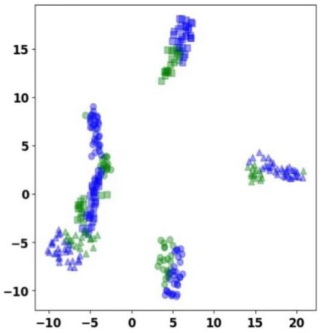
\includegraphics[width=0.32\textwidth]{chapter-2/images/tsne_SMoE.pdf}} & 
        \subcaptionbox{With SCOT-based solver.}{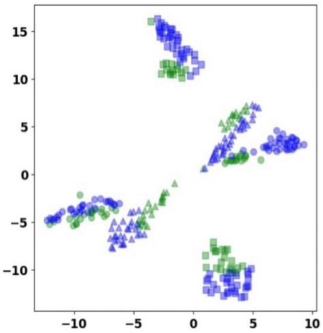
\includegraphics[width=0.32\textwidth]{chapter-2/images/tsne_SCOT.pdf}} &
        \subcaptionbox{With the proposed solver.}{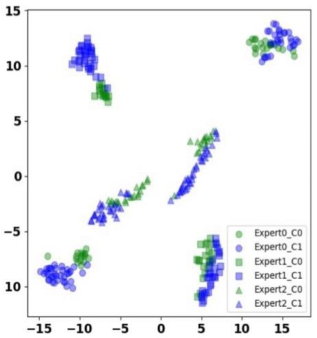
\includegraphics[width=0.32\textwidth]{chapter-2/images/tsne_proposed.pdf}}
    \end{tabular}
\caption[Evaluation of proposed Sparse-OT framework for learning a sparse-
mixture-of-experts model on a synthetic data experiment.]{t-SNE maps corresponding to the embeddings of the expert neural networks. `Expert$i\_\textup{C}j$' denotes the embeddings learnt by expert $i$ for samples belonging to class $j$. The embeddings learned with the proposed approach not only distinguish the instances from the two classes but also exhibit more diversity in terms of what each expert learns.}
\label{tsne-data1-main}
\end{figure}

\paragraph{Experimental Setup for the CIFAR Dataset Experiment.} 
Following \cite{chen2022towards}, we now use the SMoE model for a binary classification task of identifying whether a given image belongs to the CIFAR-10 dataset or the CIFAR-10-rotate dataset using a top-1 SMoE model. 
CIFAR-10-rotate consists of CIFAR-10 images, rotated by $30$ degrees. 
For SMoE, we consider four ResNet18 as the experts networks \cite{he2016residual} and train SMoEs with the gating network based on: (a) Top-1 SMoE \citep{chen2022towards}, (b) SCOT-based SMoE, and (c) the proposed Column-SparseOT-based SMoE. For both SCOT and Column-SparseOT, a sparse transport plan is learned between the $m=4$ experts and a given batch of $n$ inputs with the goal of mapping each input with only one expert ($K_2=1$). The SCOT method uses $\lambda>0$ as the coefficient of $\ell_2$ regularization.

\paragraph{Results.}
In Table~\ref{table-cifar}, we report the performance of all the three approaches. Since load balancing is an important aspect of a MoE architecture, we also report the corresponding number of inputs assigned to every expert during the inference stage. The training loss also consists of a load-balancing regularization term. We keep the coefficient of this regularization the same across the methods and also report the top-1 SMoE's performance with an increased weightage on this load-balancing factor, called Top-1 $\rm{ SMoE}_{\rm{balanced}}$.
From the results, we observe that our approach obtains a good generalization performance with balanced assignments across hyperparameters. While SCOT obtains a reasonable accuracy in one case (with $\lambda=10$), the load is not equally balanced. 
The Top-1 SMoE baseline, with the common (default) load-balancing regularization coefficient, obtains a heavily skewed allocation with two experts never getting used.
Overall, we see that our method is well suited for SMoE setting from both the generalization and load balancing points of view. 
\begin{table}[t]
\caption[Evaluation of proposed Sparse-OT framework for learning a sparse-mixture-of-experts model.]{Accuracy obtained on SMoE experiment along with the number of inputs allocated to each expert. We observe that the proposed approach obtains the best generalization performance with balanced allocation across experts.}
\label{table-cifar}
\centering
\setlength{\tabcolsep}{1.1pt}
\begin{tabular}{lcc|c|c|c}
\toprule
% Method & Accuracy & \multicolumn{4}{c}{Allocations to}\\
% & & Expert~1 & Expert~2 & Expert~3 & Expert~4\\
\multirow{2}{*}{Method} & \multirow{2}{*}{Accuracy} & \multicolumn{4}{c}{Allocations to}\\
& & \small{Expert-1} & \small{Expert-2} & \small{Expert-3} & \small{Expert-4}\normalsize\\
\midrule
    Top-1 SMoE$_{\textup{default}}$ \citep{chen2022towards} & 95.91 & 0 & 10962 & 9038 & 0\\
    Top-1 SMoE$_{\textup{balanced}}$ \citep{chen2022towards} & 93.74 & 4953 & 5018 & 4779 & 5250\\
    \midrule
    SCOT$_{\lambda=0.1}$ \citep{liu2023sparsityconstrained} & 77.96 & 3341 & 1895 & 11119 & 3645\\
    SCOT$_{\lambda=10}$ \citep{liu2023sparsityconstrained} & 90.56 & 1929 & 6112 & 6113 & 5846\\
    SCOT$_{\lambda=1000}$ \citep{liu2023sparsityconstrained} & 56.48 & 0 & 7678 & 7788 & 4534\\
    \midrule
    \rowcolor{green!10}
    Proposed$_{\lambda_1=0.1}$ & 95.56 & 5435 & 4854 & 4977 & 4734\\
    Proposed$_{\lambda_1=10}$ & 85.18 & 5000 & 5002 & 4998 & 5000\\
    Proposed$_{\lambda_1=1000}$ & 90.54 & 5000 & 5000 & 5000 & 5000\\
\bottomrule
\end{tabular}
\end{table}

\subsection{Comparing Duality Gap}\label{subsec:dualitygapcomparison}
In Sec.~\ref{subsec:partitionmatroid}, we proposed solvers for Eq.~\ref{eqn:primal} that involved maximizing a weakly submodular function under partition matroid constraints via an equivalent reformulation (\ref{eqn:reform}).
In this section, we compare the optimization quality of the proposed discrete-optimization-based approach and a continuous-optimization-based approach, discussed in Sec.~\ref{subsec:dualitygapcomparison}, which is based on the solver proposed by SCOT \citep{liu2023sparsityconstrained}.
\citet{liu2023sparsityconstrained} solve the dual of an $\ell_2$-regularized Balanced OT problem for enforcing column-wise sparsity constraints and uses a gradient-descent-based algorithm (e.g., LBFGS \citep{LBFGS}) with sparse projections to obtain the solution. We use their approach to solve Eq.~\ref{eqn:dual}, which is a dual of the primal Problem~\ref{eqn:primal}.
While Algorithm~\ref{alg:colsparseOT_dash} learns a primal solution $\bgamma_1$ of Eq.~\ref{eqn:primal}, the corresponding dual solution $\{\balpha_1,\bbeta_1\}$ can be obtained via Proposition~\ref{prop:dualitygap}. 
The SCOT approach obtains a dual solution $\{\balpha_2,\bbeta_2\}$ of Eq.~\ref{eqn:dual} and then obtains the corresponding primal solution $\bgamma_2$ by solving the sparse projection problem (\ref{eqn:conjugate}). This allows us to compare the duality gap $\Delta(\bgamma,\balpha,\bbeta) = P(\bgamma)-D(\balpha,\bbeta)$ associated with the solutions obtained by both the solvers. 

\paragraph{Experimental Setup.} We consider a uniform empirical source and target measures over two randomly chosen $100$-sized batches of CIFAR-10. The duality gap is computed over 
a range of hyperparameter $(\lambda_1,\lambda_2)$ values in Eq.~\ref{eqn:sparse-uotmmd}. The kernel used for MMD computation is fixed as the IMQ, and the hyperparameters are fixed according to the median heuristics \citep{gretton12a}.

\begin{table}[ht!]
\caption[Evaluation of the proposed Sparse-OT framework, being compared to an approximation approach for the original continuous optimization, in terms of the duality gap.]{Duality gap ($\Delta$) comparison for solving (\ref{eqn:primal}) with various hyperparameters. A lower duality gap is better. We observe that our approach obtains a lower duality gap than the SCOT-based solver.}
\label{table: main-paper-DG-imq-v2}
\centering{
% \setlength{\tabcolsep}{3pt}
\begin{tabular}{ll|cc|cc}
\toprule
\multirow{2}{*}{$\lambda_1$} & \multirow{2}{*}{$\lambda_2$} & \multicolumn{2}{>{\columncolor{green!10}}c|}{Proposed solver} & \multicolumn{2}{c}{SCOT-based solver}\\
 &  & Primal optimal obj. & Duality Gap & Primal optimal obj. & Duality Gap \\ 
\midrule
0.1 & 0.1 & \cellcolor{green!10}{$0.02993$} & \cellcolor{green!10}{$\mathbf{<10^{-10}}$}	& 0.03169	& 0.00232 \\
1 & 0.1 & \cellcolor{green!10}{$0.09183$}	& \cellcolor{green!10}{$\mathbf{0.01911}$}	& 0.27172		& 0.19111 \\
10 & 0.1 & \cellcolor{green!10}{$0.11682$} & \cellcolor{green!10}{$\mathbf{0.64896}$}	& 2.30889	& 2.21029 \\
0.1 & 1 & \cellcolor{green!10}{$0.03036$}	& \cellcolor{green!10}{$\mathbf{<10^{-10}}$}	& 0.03116	& 0.00114 \\
1 & 1 & \cellcolor{green!10}{$0.09409$}	& \cellcolor{green!10}{$\mathbf{0.00286}$}	& 0.10371	&	0.01216 \\
10 & 1 &  \cellcolor{green!10}{$0.11897$}	& \cellcolor{green!10}{$\mathbf{0.05468}$}	& 0.32334	& 0.21289\\ 
\bottomrule
\end{tabular}
}
\end{table}

\paragraph{Results.}
Table~\ref{table: main-paper-DG-imq-v2} reports the duality gap comparison with different hyperparameters. We observe that our approach outperforms the SCOT-based solver by obtaining a lower duality gap. In a couple of cases, the duality gap associated with our Algorithm~\ref{alg:colsparseOT_dash} is $< 10^{-10}$, signifying that it has converged at (or very close to) a global optimum. Additional results are discussed in Appendix~\ref{app:dualitygap}. 

\section{Conclusion}
In this chapter, we discussed the role of kernel-based squared MMD regularization for the sparsity-constrained OT problem. We established an interesting equivalence of the problem with that of maximizing a weakly submodular function over matroid constraints. We discussed novel greedy algorithms having attractive approximation guarantees for this problem. A duality gap analysis further provides an empirical way of validating the optimality of our greedy solution. Our approach also generalizes to the case of unnormalized measures, unlike the existing methods for this problem.
Experiments across different applications show the efficacy of the proposed approach.  
%A future work could be to expand on the variants of structured sparsity patterns in the OT plan.

